\title{Frequentist tests of association for imputed genotypes}
\author{Charles Zheng}
\date{\today}

\documentclass[12pt]{article} 

% packages with special commands
\usepackage{amssymb, amsmath}
\usepackage{epsfig}
\usepackage{array}
\usepackage{ifthen}
\usepackage{color}
\usepackage{fancyhdr}
\usepackage{graphicx}
\usepackage{mathtools}
\definecolor{grey}{rgb}{0.5,0.5,0.5}

\begin{document}
\maketitle

\newcommand{\tr}{\text{tr}}
\newcommand{\E}{\textbf{E}}
\newcommand{\diag}{\text{diag}}
\newcommand{\argmax}{\text{argmax}}
\newcommand{\Cov}{\text{Cov}}


\begin{abstract}
Servin and Matthews \cite{Servin2007} proposed looking for associations
between phenotypes and both typed and untyped SNPs,
by using a reference panel to infer the alleles of the untyped SNPs.
Since then, a number of GWA studies have reported \emph{p}-values for both
typed and untyped SNPs.
However, results of Almeida \emph{et al}\cite{Almeida2011} indicate
that using imputed genotype data can lead to increased type I error.
We discuss possible causes of inflated type I error from using
imputed data and propose methodology designed for conducting GWAS
studies with imputed genotypes.

\end{abstract}

\section{Introduction}

A primary focus of genetics is the identification of
the genetic variants causing variation in a particular
phenotype of interest, such as height, susceptibility to diabetes,
or drug sensitivity.
The earliest discoveries of such genetic variants were made by 
linkage analyses--studies which compared genotypes within the same
family.
However, such studies failed to discover variants accounting
for the genetic basis of complex diseases such as diabetes.
This led geneticists to suspect that the genetic component of complex diseases
were distributed among many genes with small effects on
disease susceptibility.
As Risch and Merikangas noted in their seminal paper \cite{Risch1996},
it would be very difficult to discover such small-effect variants
with linkage studies; however, it could be much more feasible
to discover such variants by carrying out association studies on
unrelated individuals.

Indeed, Risch and Merikangas anticipated the introduction of the genome-wide
association (GWA) study.
In a GWA study, the genotypes
 of possibly unrelated case and control subjects
are compared to find associations between
phenotypes and genetic variants: single-nucleotide polymorphisms
(SNPs) or less commonly, copy-number variations \cite{Clarke2011}.
Such associations can help narrow the search for the true causative
variants:
due to the strong correlation between variants located close to one
another on a chromosome (linkage disequilibrium), a causative variant
will induce associations between nearby variants and the
phenotype.
That said, not all putative associations found in GWA studies
are necessarily induced by linkage disequilibrium with a causative variant:
many could be caused by population stratification, sampling biases,
or false positives
\cite{Pearson2008}.
Despite these shortcomings, researchers have suceeded in using GWA
studies
to uncover interesting genetic variants involved in important
diseases, including type I diabetes and Crohn's disease \cite{Visscher2012}.

A major component to the cost-effectiveness of GWA studies is
the fact that interesting discoveries can be made by
sequencing a relatively small subset of the  subjects' genomes.
Thus GWA studies typicially rely on tag-SNP chips which allow them
to cheaply sequence on the order of 300,000 sites in the genome.
These tag-SNP sites are chosen to exploit the block patterns
found in human genetic variation.
As discovered in the HapMap project, 5-15 kilobase blocks
of alleles, or haplotype blocks, tend to be coinherited--
and the diversity of haplotype blocks in a given population
can be quite low \cite{HapMap2007}.
Meanwhile, the tag SNPs are chosen to optimally distinguish common
haplotypes for each block.
Therefore, causative variants included in a common haplotype
will likely induce an association between the tag SNPs chosen
for that block.

Interestingly, though, due to the availability of population-level
SNP and whole-genome data provided by sequencing efforts such as HapMap and
the 1000 genomes project, it is possible to accurately impute many
additional SNPs of a subject from their genotyped SNPs.
Servin and Matthews \cite{Servin2007} proposed a statistical
framework to find associations between the phenotypes and the imputed
SNPs in addition to the typed SNPs, which could possibly lead to more
discoveries.
Almeida \emph{et al.} \cite{Almeida2011} investigated the reliability of
results obtained from imputed SNPs.
Using case-control data from a type I diabetes study, they compared
p-values obtained from a set of genotyped SNPs
with p-values obtained from imputed values from the same SNPs.
They found that less than half of the imputation-based p-values below the
threshold of $10^{-5}$ had corresponding genotype-based
p-values below the threshold, and concluded that the use of imputed
SNPs leads to an inflated type I error rate.
Nevertheless, a number of recent meta-analyses
\cite{Dupuis2010}\cite{Levy2009} have used imputed SNPs.

Since Sevin and Matthews first proposed the analysis of imputed SNPs,
a number of algorithms for genotype imputation have been developed.
The most recent algorithms can automatically find boundaries of
haplotype blocks, as well as automatically perform phasing on both
reference panel data and case/control data.
Marchini and Howie \cite{Marchini2010} provide a detailed review of the most
popular algorithms.

\subsection{Statistical Evaluation}

An extensive body of frequentist statistical literature applies to
GWA studies using only genotyped SNPs \cite{Ziegler2008}.
Chiefly, there exist two major methodologies for multiple testing
which can be applied to interpret the p-values obtained
from genotyped data: the Bonferroni procedure,
which controls the the family-wise error rate (FWER)
and the Benjamini-Hochberg (BH) procedure,
which controls the false discovery rate (FDR) \cite{Storey2003}.
But while the majority of GWA studies do use marginal association
tests for the individual SNPs, whether genotyped or imputed,
most do not bother to apply either multiple testing procedure,
instead reporting \emph{p}-values below a prespecified threshold, e.g.
$10^{-5}$.

A major reason for this practice is that the unmodified Bonferonni and BH
procedure are overly severe when dealing with large numbers
of highly correlated test statistics.
Lin \cite{Lin2005} and Dudbridge \cite{Dudbridge2006} have suggested
using permutation-test based modifications to the Bonferonni or BH
procedure which ameliorate the effect of high correlations on
statistical power.
Storey and Tibshriani \cite{Storey2003} also propose
a permutation-test based procedure to control false discovery rate,
which is theoretically conservative under ``weak dependence''
conditions.
We go into more detail about these modified Bonferonni and BH
procedures in Section 2.

But moreover, as Ziegler \emph{et al} note, neither the control of FWER
nor FDR
``overcome the fundamental problem that formal statistical testing often
is not the primary aim in a GWA...[which is] to know whether a SNP is
worthy of further investigation...''

Indeed, even supposing that such frequentist procedures are
theoretically effective for detecting associations,
there is the additional issue that such theoretical properties
depend on a ``sparse effects'' assumption in which all uninteresting
SNPs have zero association with the phenotype.
Yet this assumption is most definitely violated in practice:
recall that any SNPs in linkage disequilibrium with a causative variant
would have association with the phenotype will formally
be considered non-null features.
Thus neither frequentist procedure is guaranteed to control
the number of such SNPs reported.
This is a minor issue if such SNPs are close to the causative SNP,
but Reich \emph{et al} \cite{Reich2001} find that within the European population
regions of detectible linkage disequilibrium routinely extend to 160
kilobases around an SNP.
Given the effort required to hunt for a causative variant
in a 5 kb region, one would surely consider an SNP which is 160 kb
away from a causative variant to be uninteresting; yet
the established framework for multiple testing makes no special
provision to exclude such hits.

For these and other reasons, 
many statisticians have proposed abandoning single-marker analysis altogether,
advocating regression \cite{Frommlet2010} or other machine
learning-based approaches, or Bayesian inference \cite{Servin2007}.
Such alternative approaches generally have a shorter history than
the body of frequentist work: significance testing for
high-dimensional regression is currently an extremely active area of
research,
with many new approaches proposed within the last two years
\cite{Bogdan2013}\cite{Javanmard2013}\cite{Taylor}.
Bayesian modelling approaches, though already quite complicated,
still have enormous room to grow, including incorporation
of population structure \cite{Stephens2009}.

While both acknowledging the known disadvantages of single-marker-based
frequentist analysis and the promise of alternative methodologies to
GWA studies, we will consider the possible use of the multiple-testing
framework on both genotyped and imputed SNP data in the rest of the
paper.

As we mentioned, a major shortcoming of the current multiple testing
framework is the fact that it fails to formally discriminate between
SNPs strongly associated with the phenotype and SNPs very weakly
associated with the phenotype.  
A second major shortcoming of the current body of frequentist
methodology is the lack of a framework for dealing with imputed data.

However, we feel that both of these shortcomings can be overcome,
and in this paper, we will discuss possible ways to do so.
If, indeed, a satisfactory frequentist testing procedure can be
developed which overcomes these shortcomings while maintaining
an adequate power,
the use of such a procedure in GWA studies would yield
an important benefit:
a metric to gauge the reliability of putative
associations.
Researchers
would be able to use these frequentist measures to inform
their decisions on whether or not to follow up on the SNPs found
by a particular study or meta-analysis.

The first shortcoming of the frequentist approach, which is its failing to
distinguish between strong and weak effects,
can be addressed in a number of ways.
One approach, proposed by Wager \cite{Wager2013a} in an
unpublished
paper, is to define an ``irrelevance coefficient'' which penalizes
features with small effects, and to control the average
irrelevance coefficient of the reported features
analogously to how the BH procedure controls the average proportion
of false discoveries within the reported features.
For reasons of convenience, we take a simpler approach,
which is to redefine a null feature to be one with a possibly
nonzero effect which falls below a threshold.
The effect of this on existing procedures is to modify
the method of computing $p$-values.

Under this new perspective, a Type I error
corresponds to misclassifying a weak effect as a strong effect.
This corresponds more closely to scientific realities,
in which the discovery of a weakly associated SNP is not much
preferable to the discovery of an unassociated SNP.
Existing procedures will continue to control the Type I error
given the modified method of computing $p$-values when using genotyped
data.
However, an increased Type I error rate (in the form of increased FWER
or increased FDR) can still occur if the Bonferroni or BH procedure
are used on imptued data.

In this project,
we explore population-level phenomenona which could lead
to failures of the Bonferroni or BH method
are naively applied to imputed SNPs;
additionally, we suggest a novel statistical procedure
designed specifically for carrying out hypothesis testing with imputed
data,
which continues to incorporate the threshold-based definition
of a null hypothesis.

\section{Testing of associations in genotyped data}

Let $\mathcal{S}= \{s_1,\hdots,s_M\}$ be a set of biallelic SNPs of interest,
and let us fix a reference haplotype.
Let $(Z,X^{(1)}, X^{(2)})$ be random variables representing
a phenotype $Z$ taking values $\{0,1\}$ and two haplotypes $X^{(1)}, X^{(2)}$ for individuals
in a population, where $X^{i,(j)}$ is the value of the SNP $s_i$ in
the $j$th haplotype; $X^{i,(j)}=0$ if the SNP has the same allele as
the reference.

We obtain data for $L$ cases and $L$ controls
in the following manner.
We sample the cases as iid draws from the population
conditional on $Z=1$, and the controls as iid draws
conditional on $Z=0$.
Given this sampling, we obtain genotypes
$X^{(1)}_1,X^{(2)}_2,\hdots,X^{(1)}_L,X^{(1)}_L$ for
controls
and $X^{(1)}_{L+1}, X^{(2)}_{L+1},\hdots,X^{(1)}_{2L},X^{(2)}_{2L}$
for cases.
These genotypes could variant calling or phasing errors,
but we will assume that such errors
affect cases and controls in the same way.

Given this data, we compute for each SNP $s_i$ the total minor allele count
for cases $T_i$ and the total minor allele count for controls $U_i$,
\[
U_i = \sum_{k=1}^{L_0} X^{i,(1)}_k + X^{i,(2)}_k
\]
\[
T_i = \sum_{k=L_0+1}^{L} X^{i,(1)}_k + X^{i,(2)}_k
\]
Given this, we compute the empirical log-odds ratio $\hat{\theta}_i$ for the $i$th SNP:
\[
\hat{\theta}_i = \log(T_i) - \log(2L_1- T_i) + \log(2L_0-U_i) - \log(U_i),
\]
an estimate of the true log-odds ratio $\theta_i$,
and the empirical variance\cite{Morris1998} of the estimate:
\[
V_i = \frac{1}{U_i} + \frac{1}{2L_0 - U_i} + \frac{1}{T_i} + \frac{1}{2L_1-T_i}
\]

Now we set a threshold $\tau$ for ``small-effect'' SNPs, e.g. $\tau=0.05$.
For low $\tau$, SNPs with odds ratios between approximately $1-\tau$
and $1+\tau$ will being classified as ``small-effect''.
Setting $\tau=0$ recovers the standard paradigm of hypothesis testing
where null SNPs have odds ratios of exactly 1.
A type I error corresponds to reporting such a ``small-effect'' SNP.

Given only a specification of $\tau$, we can compute the raw
$p$-values
to be used in the multiple testing procedure as
\[
P_i = 2-2\Phi\left(\frac{(\hat{\theta}_i-\tau)_+}{\sqrt{V_i}}\right)
\]
where $(x)_+ = xI(x > 0)$ and $\Phi$ is the normal cumulative distribution function.

After obtaining the raw $p$-values,
any of the multiple testing procedures \cite{Lin2005}
\cite{Dudbridge2006}
\cite{Storey2003}
can be applied to assess the statistical significance of
the findings.

In the paper we will mainly focus on the use of the original
Benjamini-Hochberg procedure \cite{Benjamini1995}:
\[\]
\noindent\textbf{BH procedure}
\begin{enumerate}
\item Fix a false discovery rate threshold $q$
\item Given $p$-values $p_1,\hdots,p_M$, sort them in ascending order:
\[
p_{(1)} \leq p_{(2)} \leq \hdots \leq p_{(M)}
\]
\item 
Compute $t_1,\hdots,t_M$
by $t_i = \frac{M}{i}p_{(i)}$
\item Let $j$ be the largest index such that $t_j \leq q$
\item Let $p_{c_1},\hdots,p_{c_j}$ be the $j$ smallest $p$-values.
Report the SNPs $s_{c_1},\hdots,s_{c_j}$.
\end{enumerate}
Let $V$ be the number of null SNPs reported, and $R$ the total
number of null SNPs reported.
Then the false discovery rate (FDR) is $\textbf{E}[V/R]$,
where the expectation is taken over the sampling distribution of the data.
The BH procedure has the property of controls the false discovery
rate, i.e.
\[
\textbf{E}\left[\frac{V}{R}\right] \leq q
\]

\section{Naive Testing of Imputed Data}

Now we consider what could go wrong if the procedure
outlined in section 2 is applied to imputed data.
We modify the setup of section 1 by supposing that a reference panel
is available for the full set of SNPs $\mathcal{S}$, but that
only a
subset $\mathcal{S}_{tag}$ of the SNPs are observed for the case and
control data:
without loss of generality, let $s_1,\hdots,s_N$ be the observed SNPs.
Here we are assuming that the observed genotypes are correctly phased:
again, this is an assumption made for the sake of discussion,
and in reality there would be additional issues due to the uncertainty
of phasing.

The reference panel gives rise to an imputation rule $\hat{Q}$,
a function of a haplotype containing observed SNPs.
While results may differ depending on the particular imputation rule,
we claim that the most widely used approaches \cite{Marchini2010}
can be interpreted as methods to estimate the conditional joint
distribution of a haplotype in the reference population
given its observed elements
\[
\hat{Q}(X^{(j)}|X^{1,(j)},\hdots,X^{N,(j)}) \approx \Pr[X^{(j)}|X^{1,(j)},\hdots,X^{N,(j)}]
\]
In fact, an idealized imputation rule would replicate the distribution
precisely, while a ``good'' imputation rule would differ slightly
from the true conditional distribution.
However, as we will demonstrate, even an idealized imputation
rule can lead to type I error due to differences between
the reference population and the case or control populations.

Given such an imputation rule, Guan and Stephens \cite{Guan2008}
describe procedures to generate either Bayes factors or
likelihood-ratio-based test statistics which take into account
the uncertainty of the imputation.
They also conclude that in the Bayesian framework,
similar performance can be obtained by
using the posterior mean of the conditional distribution.
However, recent studies \cite{Dupuis2010}\cite{Levy2009}
suggest that the current practice in meta-analyses
is to directly impute SNPs, apply quality filters,
and then apply standard association tests
as the imputed values were real data.
Hence in the following, we will consider using the posterior mean imputed
values,
and then naively applying the procedure in section 2:
we feel that such a procedure is only a slight modification of current
practice.

To elaborate, given the imputation rule $\hat{Q}$, interpreted
as an estimate of the conditional probability distribution
of the untyped SNPs in the reference population,
we produce imputed haplotypes
$\tilde{X}^{N+1,(j)}_i,\hdots,\tilde{X}^{M,(j)}_i$
for each individual $i$ and haloptype $j$,
by
\[
\tilde{X}^{k,(j)}_i = \hat{Q}(X^{k,(j)}=1|X^{1,(j)}_i,\hdots,X^{N,(j)}_i)
\]
Then the procedure in section 1 is applied, as if the imputed
haplotype
$\tilde{X}^{(j)}$ was originally observed.

The question we now consider is: under what conditions
will this naive protocol lead to an increased type I error,
in the form of either increased FWER or increased FDR?

\emph{Remark.}
Recall that in this context, an increased type I error
means misclassifying an SNP with small effect (that is,
with absolute log-odds less than $\tau$)
as an SNP with non-small effect.
If $\tau=0$, corresponding to the classical definition of null
hypothesis,
the question has a trivial answer,
since for any SNP associated with the phenotype,
all SNPs in linkage disequilibrium with the SNP will also
be associated with the phenotype, and hence be considered non-null.
The only source of increased type I errors is if an
SNP independent of the phenotype has a different imputed-value
distribution
between cases and controls.
Yet, in order for the SNP to have a different imputed-value
distribution,
there must exist at least one other SNP must be considered to be in LD
with the null SNP (according to the imputation rule $\hat{Q}$) which has an association with the phenotype.
Yet, in reality, it is not possible for there to exist any SNP
associated
to the null SNP which is associated with the phenotype.
\textbf{Therefore, under the classical definition of null hypothesis,
increased type I error is only possible when the imputation
rule $\hat{Q}$ erroneously attributes dependence between two independent SNPs.}
But some population-genetics assumptions would make the
problem of failing to capture independence relationships a practical non-issue.
It is generally realistic to assume that the reference population
contains the case and control populations as subsets,
and furthermore, that the reference population is more ``diverse.''
In particular, we would assume that any pair of SNPs which are
independent
in the case or control population are independent in the reference
population.
Supposing this is the case, then the risk for increased type I error
is mitigated if the imputation algorithm captures the
haplotype block structure accurately: a task which many algorithms
can accomplish fairly well \cite{Stephens2005}.
It is important to note, though, that for $\tau > 0$,
the problem of controlling type I error becomes much more challenging,
and even an idealized imputation rule
can lead to increased type I error.

Given the threshold-based definition of null SNPs, we note the
following
possible causes of increased type I error.
\begin{enumerate}
\item \emph{Miscalled SNPs.}
Miscalled variants in the typed SNPs could lead to incorrectly
imputed posterior means in the untyped SNPs.
Almeida \emph{et al} \cite{Almeida2011} noted that filtering for
variant call quality improved the agreement between imputed $p$-values
and $p$-values obtained from genotyped data.
\item \emph{Inaccuracies in imputation rule relative to reference.}
A low sample size for the reference population
limits the accuracy of the derived imputation rule,
especially if haplotypes common in either the case or control
but rare in the reference population are not included
in the reference panel.
If two SNPs are weakly asssociated in $\hat{Q}$ but strongly
associated in the reference population, this not lead to increased type I errors,
since weak associations in the imputation rule tend to lead to imputed
allele sums being similar in cases vs controls.
Increased type I error could more likely occur if
two SNPs strongly associated in $\hat{Q}$
are in reality weakly associated.
Suppose the imputation rule contains a strong association between
a typed SNP $s_s$ strongly associated with a phenotype
and an SNP $s_w$ very weakly associated with the phenotype,
but in the control and/or case population, $s_s$ is only weakly
associated with $s_w$.
Then the difference in case counts of $s_s$ and control counts of
$s_s$
would lead to a significant difference in imputed sums of $s_w$ in
the cases vs controls, when in reality the ratios of sums in cases vs
controls is much closer to 1.
\item \emph{Mismatch between the reference and study population.}
Even supposing the imputation rule is quite faithful to the reference
population,
there may be a mismatch between the reference population and study
population
from which cases and controls are drawn.
If the reference population contains a strong association between
a typed SNP $s_s$ strongly associated with a phenotype
and an SNP $s_w$ very weakly associated with the phenotype,
but in the control and/or case population, $s_s$ is only weakly
associated with $s_w$, this could lead to increased type I error,
for the same reasons as mentioned immediately above.
\item \emph{Population-level causes.}
Even with a reference panel derived from the same population as the controls,
and an idealized imputation rule,
increased type I errors could still occur.
See next subsection.
\end{enumerate}
Before we move on for a more detailed discussion of population-level
causes,
we remark on a counter-intuitive aspect of the problem.
Note carefully that an inadequate sample size does \emph{not} appear
on the list for possible reasons of increased type I error.
This is because frequentist procedures automatically account
for the increased variance due to low sample size--that is,
until the sample size begins to cause violations to
crucial assumptions such as normality of the test statistics.
However, since the procedures do \emph{not} account for
possible errors due to imputation,
type I error for imputed SNPs may, indeed, increase dramatically
as sample sizes increase.
This is because the only way for a type I error to occur
is for the erroneous signals in the imputed SNPs to gain sufficient
strength
to overcome the $p$-value threshold used.

\subsection{Population-level causes of increased type I error}

Suppose that the reference and control population are the same,
and the imputation rule $\hat{Q}$ captures the true
conditional distribution of haplotypes in the control population.

We provide a scenario to illustrate how a type I error can still
occur.
Consider a haplotype block with 5 SNPs, labeled A, B, C, D, E (Fig .1)
Only B, C, and D have strong associations with the phenotype.
Note that while in the figure, E appears to have an odds ratio of
zero,
this is only due to the discreteness of the example:
realistically, in a large population of cases and controls,
it would have true odds ratio close but not equal to zero.
A reference panel provides the joint distribution of all five SNPs.
However, only A, B, and C are genotyped for cases and controls.
The distribution of haplotypes within the haplotype block
for the control population is very similar to the distribution
for the reference population.

\begin{figure}[h]
\centering
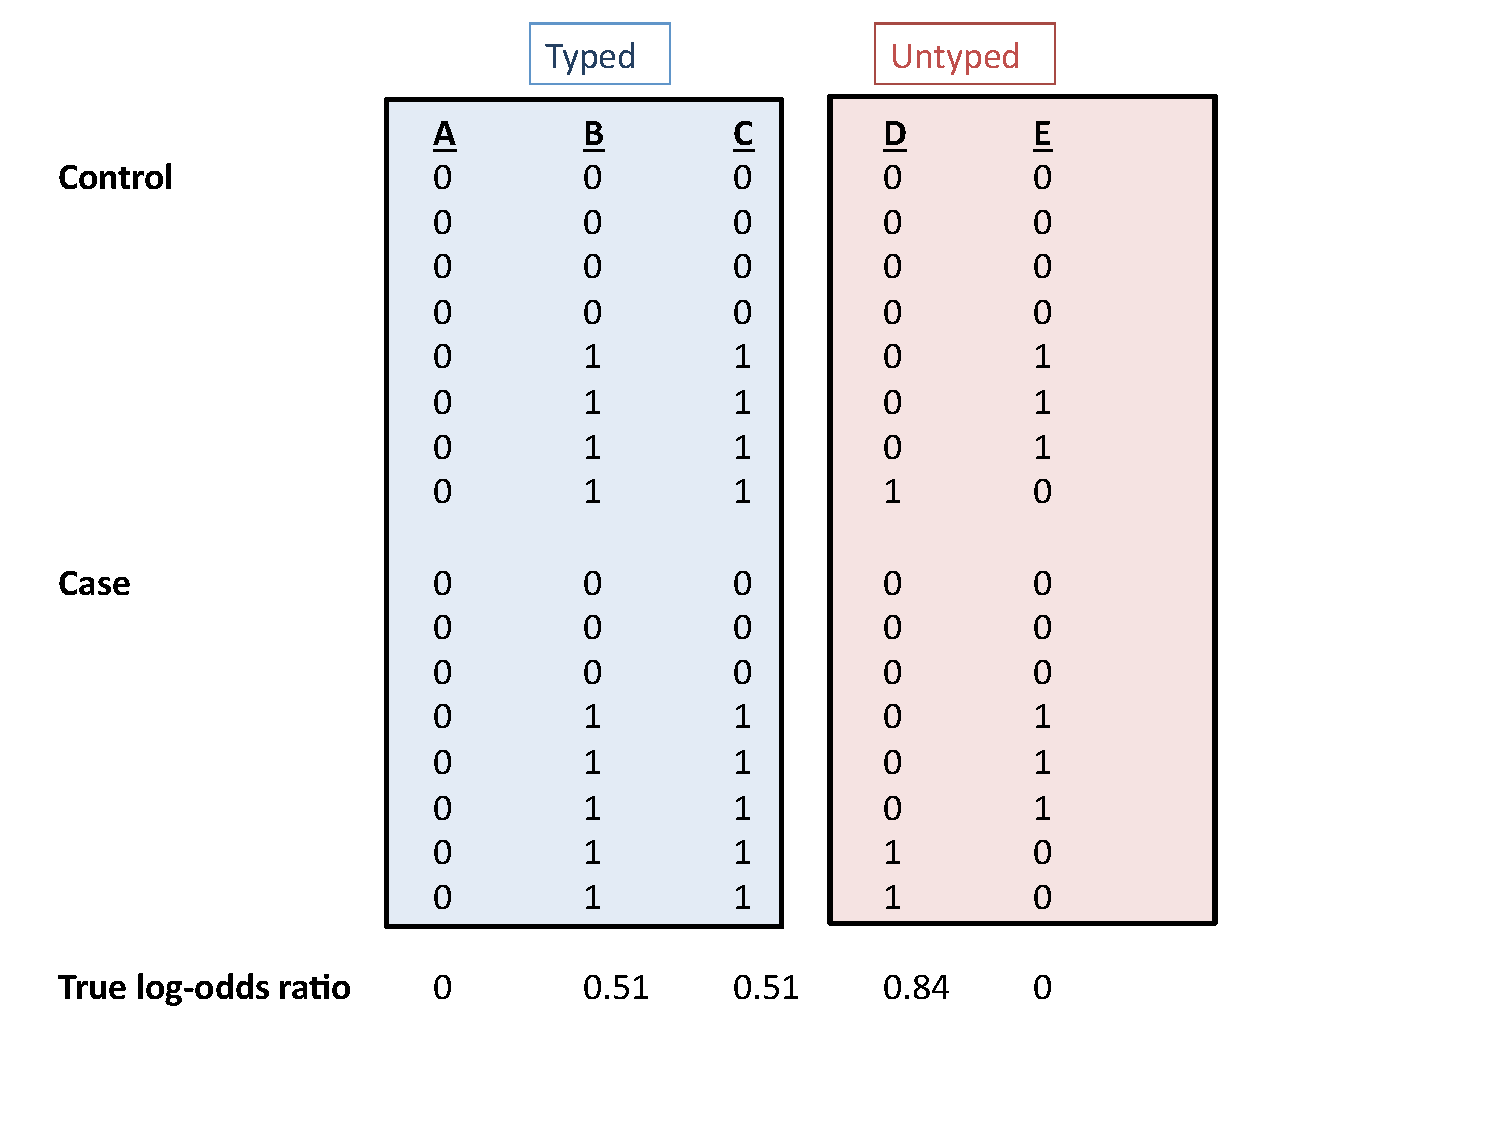
\includegraphics[scale=0.5]{impute_fig1.pdf}
\caption{True distribution of case and control population}
\end{figure}

Given a sufficiently large sample size,
the proportions of the haplotypes in the case and control samples
will closely match the population-level distributions shown in Fig 1.
But when this is the case, the estimated log-odds ratio for E will be much
larger than than the true log-odds ratio, leading to a type I error:
this is illustrated in Figure 2.

\begin{figure}[h]
\centering
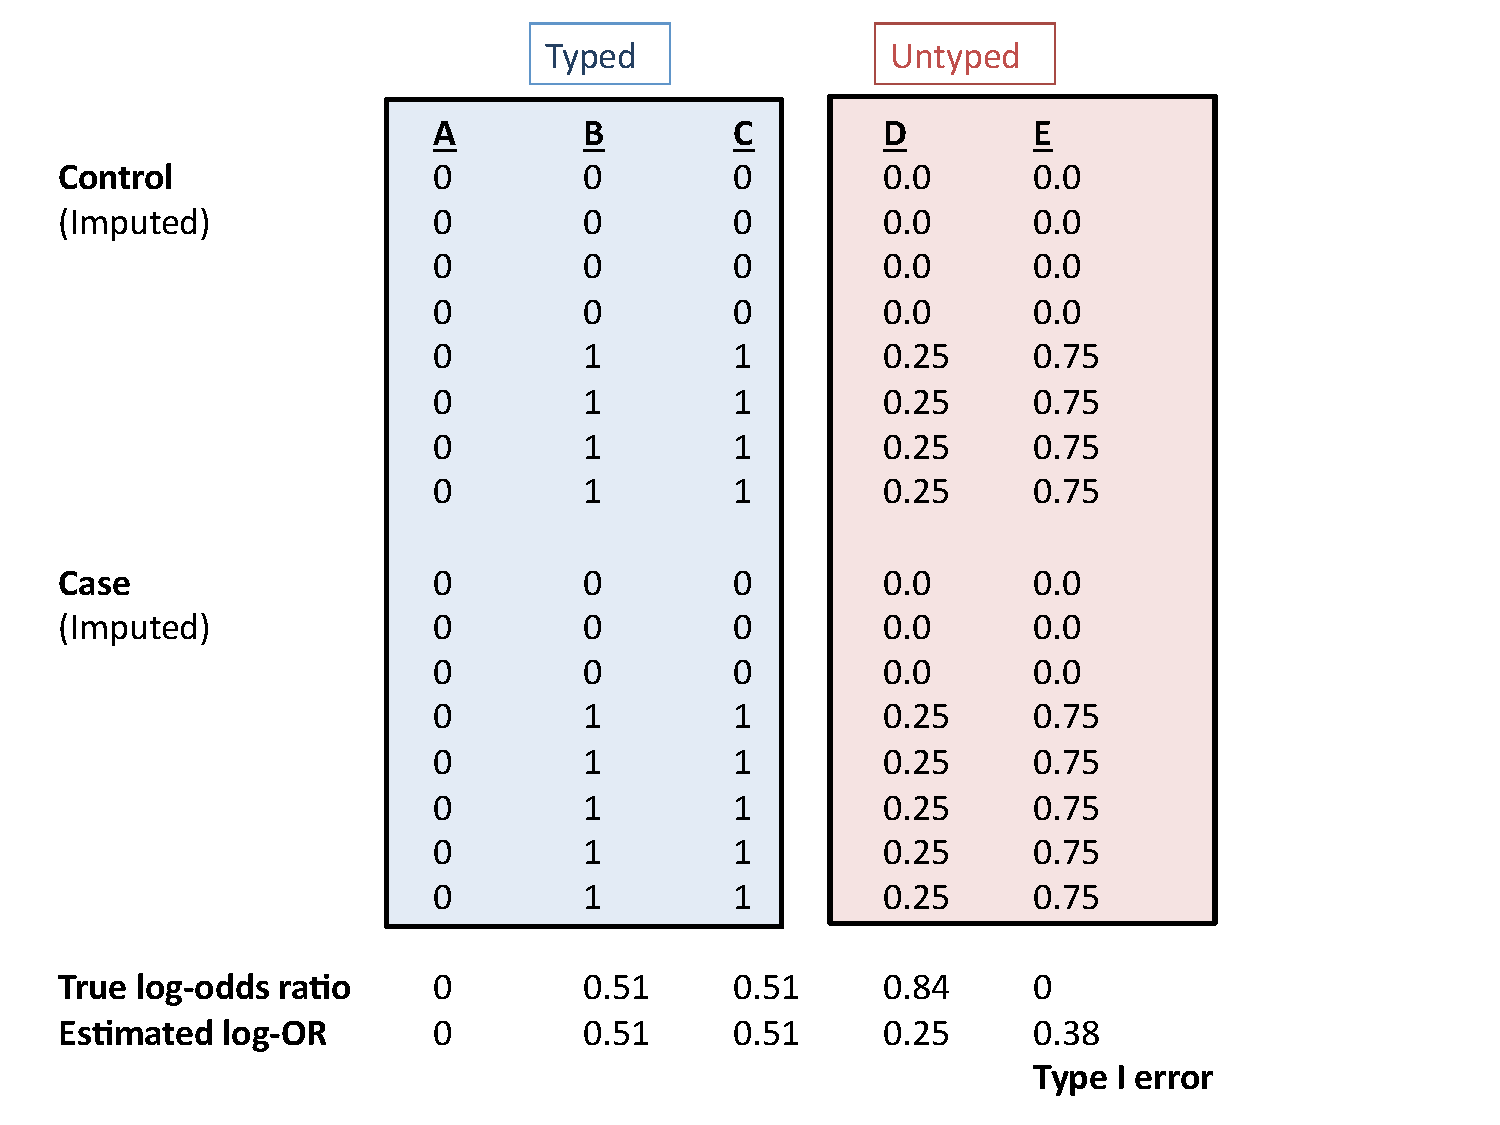
\includegraphics[scale=0.5]{impute_fig2.pdf}
\caption{Estimated log-odds ratios of imputed SNPs}
\end{figure}

We can generalize this simple example to understand
a class of patterns which would give rise to type I errors
for imputed data
\emph{which are intrinsic to population-level
distributions of haplotypes for the cases and controls}.
In the example, there are three haplotypes, which we call
$\alpha,\beta,\gamma$:
\begin{align*}
\alpha : & (00000)\\
\beta : & (01110)\\
\gamma : & (01101)
\end{align*}
Note that crucial to this example is the fact that $\beta$
and $\gamma$ are indistinguishable given the typed SNPs,
and that $\gamma$ is much more rare than $\beta$
in the control population.
Yet, $\gamma$ is enriched in the case population,
while $\beta$ is not.
A possible mechanism is that the minor variant for SNP E,
which is unique to haplotype $\gamma$,
is a causative variant for the phenotype.
The final ingredient is the fact that the minor variant for SNP D
is unique to $\beta$.
Otherwise, if SNP D was also present in haplotype $\gamma$,
while the SNP may not be causative, it would still be associated
with the phenotype, and still technically count as a true positive.

We generalize the example to a class of population-level patterns
leading to type I errors:

\noindent\textbf{Pattern I}
\begin{enumerate}
\item There exist two haplotypes $\beta, \gamma$ for a given haplotype
  block,
which are indistinguishable given the typed SNPs.
\item The haplotype $\gamma$ is enriched in either the case or control population,
while $\beta$ is enriched in neither the cases nor controls.
\item The haplotype $\beta$ contains minor variants not present in
  $\gamma$,
nor any other haplotype which is enriched in the case population.
\item The haplotype $\beta$ is relatively common in the reference
  population, while $\gamma$ is rare.
\end{enumerate}

This effect can persist
even if there exist other haplotypes $\delta,\epsilon$ etc.
possibly also containing SNPs associated with the phenotype,
as long as the total increase in rare haplotypes in
the case population relative to the reference population remains
small relative to $\tau$.

We suggest a plausible geneological mechanisms for
how such haplotypes $\beta,\gamma$ could arise within a haplotype
block in Figure 3.
Initially, a common ancestor $\zeta$ of both $\beta$ and $\gamma$
propagates.
Both the $\beta$ and $\gamma$ haplotypes emerge;
but somehow, the $\beta$ haplotype ends up occupying a large
proportion
of the haplotypes descended from $\zeta$.
Crucially, the mutation associated with the $\gamma$ haplotype
does not reappear, in a large fraction, in any of the $\beta$
haplotypes.
Such a process could occur, in parallel, over all of the haplotype
blocks in the genome.

\begin{figure}[h]
\centering
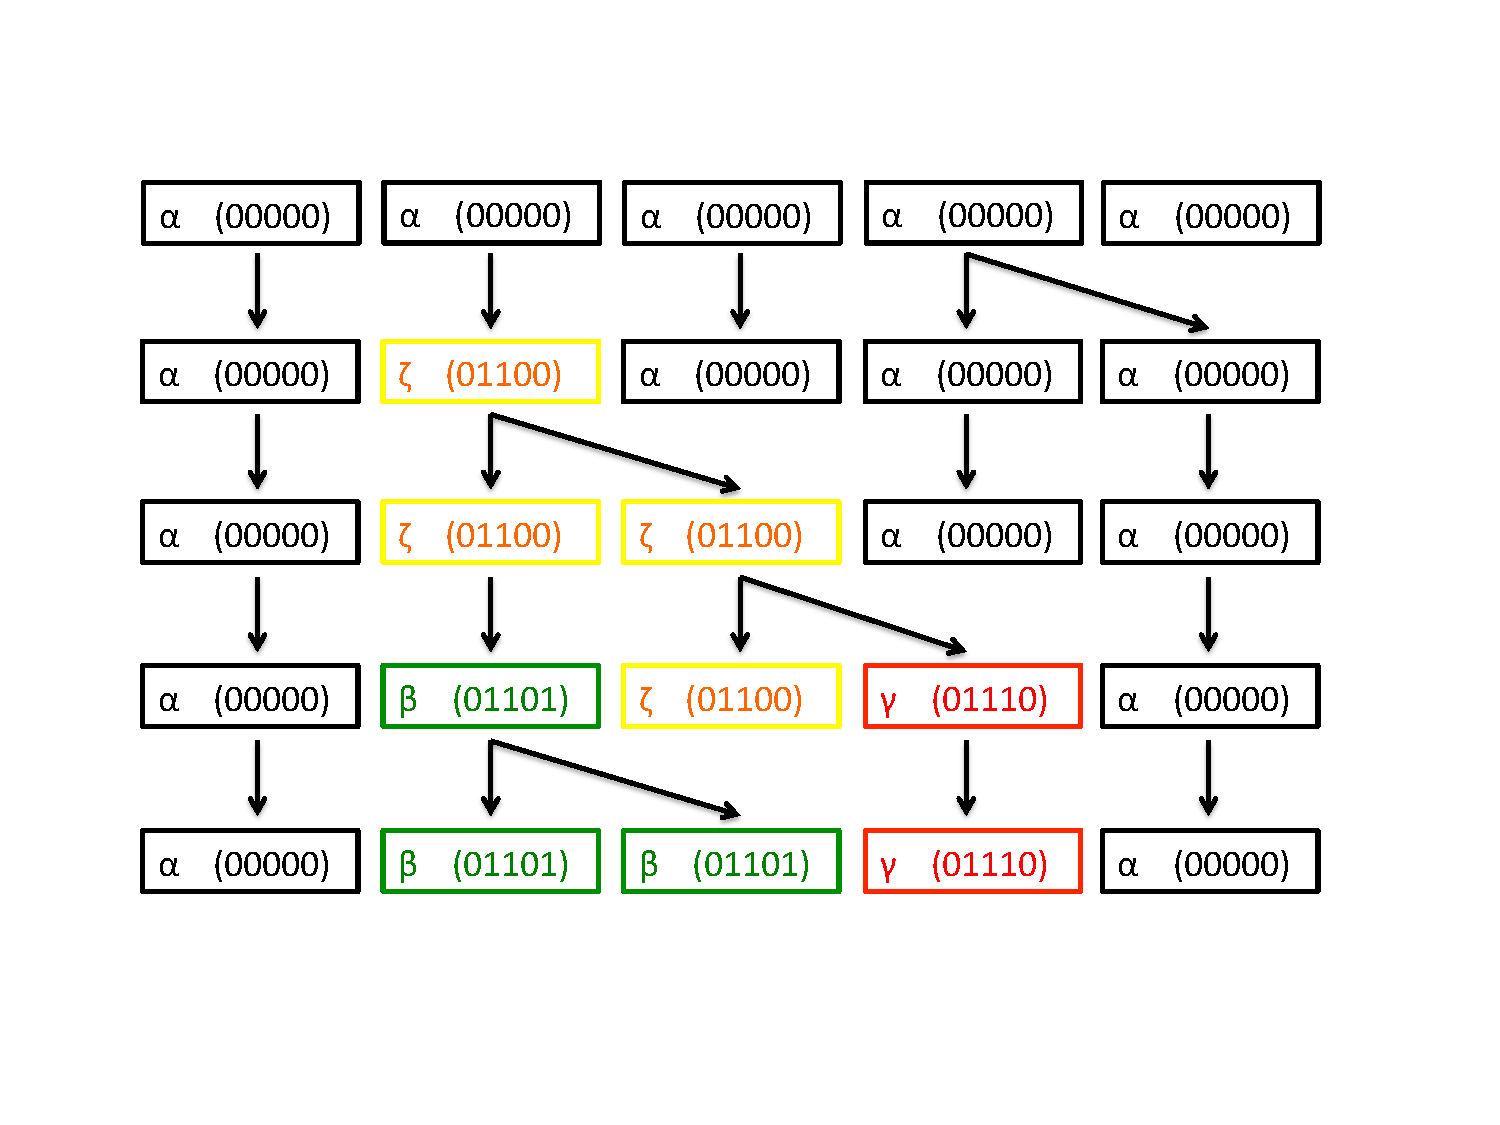
\includegraphics[scale=0.5]{impute_fig3.pdf}
\caption{Possible geneological mechanism for Pattern I}
\end{figure}

Still, the actual impact on type I error rates depends on
the relative fraction of haplotype blocks containing such
$\beta$,$\gamma$ haplotypes.
It would be interesting, and perhaps informative, to assess the
likelihood of Pattern I arising in a population genetics
framework, in relation to the number of typed SNPs.
If the prospect is relatively unlikely given a decent number of typed SNPs this would indicate less need for
caution in testing imputed data.
All the same, we show in the next section that it is possible
to get guaranteed type I error control for imputed data.

\section{A nonparametric method for testing associations in imputed data}

The fundamental problem with naively applying a multiple testing
method
to imputed data is that the implicit assumption that the imputation
rule captures the dependency structure of the cases and controls.
When this assumption is violated, there is no guarantee of type I
control.
However, we can test the validity of this key assumption
by paying an extra price:
genotyping a larger set of SNPs on a \emph{validation sample}.

Using this idea, we develop a method for testing associations in imputed
data which can deal with all of the possible causes of failure
listed in section 3: miscalled SNPs, inaccurate imputation rule,
mismatch between reference and control, and population-level causes.

\subsection{Procedure}

Let us continue with the setup of section 3.
This time, in addition to collecting a subset $\mathcal{S}_{tag}$
on $L$ individuals,
we will sequence an additional $L_{val}$ individuals.
From this validation sample, we genotype both $\mathcal{S}_{tag}$ and 
an additional set of validation SNPs $\mathcal{S}_{val}$.
The set of validation SNPs is randomly selected from the set of SNPs
of interest, minus the tag SNPs.
That is, letting $N_v$ be the number of validation SNPs,
\[
\mathcal{S}_{val}= \{s_{I_1},\hdots,s_{I_{N_v}}\}
\]
where $I_1,\hdots,I_{N_v}$ are selected uniformly at random
without replacement from $N+1,\hdots,M$.

Our data is as follows:
\begin{itemize}
\item A reference panel, which yields an imputation rule $\hat{Q}$.
\item Phased genotypes for $\mathcal{S}_{tag}$ from $L$ cases and $L$ controls
\[
X_i^{1,(1)},X_i^{1,(1)},\hdots,X_i^{N,(1)},X_i^{N,(2)}
\]
with $i=1,\hdots,L$ for controls and $i=L+1,\hdots,2L$ for cases.
\item Phased genotypes for $\mathcal{S}_{tag}$ and randomly selected
  validation SNPs $\mathcal{S}_{val}$ from $L_{val}$ cases and
  $L_{val}$ controls
\[
X_i^{1,(1)},X_i^{1,(1)},\hdots,X_i^{N,(1)},X_i^{N,(2)},
X_i^{I_1,(1)},X_i^{I_1,(2)}\hdots,X_i^{I_{N_v},(1)},X_i^{I_{N_v},(2)}
\]
\item Imputed genotypes for $L$ cases and $L$ controls,
  $\tilde{X}_i^{(j)}$
for $i = 1,\hdots,2L$ and $j=1,2$.
\end{itemize}

Our procedure involves two control parameters, $\alpha_1$,
$\alpha_2$, in addition to the discovery threshold
$\tau$.
We will make use of the assumption that the true number of null SNPs
is greater than the true number of alternative SNPs.
\[\]
\noindent\textbf{Procedure for Imputed Genotypes}
\begin{enumerate}
\item Conduct the standard testing procedure for the tag SNPs on combined
sample of $L+L_{val}$ cases and $L+L_{val}$ controls as a separate analysis
\item Obtain $p$ values for validation SNPs
\[\mathcal{P}^{val} = \{p^{val}_{I_1},\hdots,p^{val}_{I_{N_v}}\}\]
using the formula presented in section 2
\item \emph{(BH procedure for validation data)} From the validation data, we will obtain a set of
  \emph{presumed null} SNPs.
Apply original BH procedure\cite{Benjamini1995} with $q=0.5$ to $\mathcal{P}^{val}$.
Define the set of presumed nulls 
\[\mathcal{S}_{prenull} = s_{J_1},\hdots,s_{J_A}\]
as the subset of validation SNPs \emph{accepted} by the BH procedure.
\item Obtain imputed $p$ values for the $L$ cases and $L$ controls
  $\tilde{p}_1,\hdots,\tilde{p}_M$.
\item The set of imputed $p$ values for $\mathcal{S}_{prenull}$
\[
\tilde{\mathcal{P}}_{prenull} = \{\tilde{p}_{J_1},\hdots,\tilde{p}_{J_A}\}
\]
will be used to estimate the distribution of the imputed $p$ values
of the null SNPs.
\item Given $\tilde{\mathcal{P}}_{prenull}$ and parameter $\alpha_1$,
obtain a set of transformed imputed $p$-values for the untyped
  SNPs $\mathcal{S}_{imputed} = \mathcal{S}\setminus\mathcal{S}_{tag}$,
\[
\hat{p}_i = \hat{L}(\tilde{p}_i)
\]
for $i = N+1,\hdots,M$ (details in next section).
\item \emph{(BH procedure for main data)} Apply the original BH procedure with $q =\alpha_2$ to the
  transformed $p$ values $\hat{\mathcal{P}} =
  \{\hat{p}_{N+1},\hdots,\hat{p}_M\}.$
Report the SNPs rejected by the BH procedure for the main data.
\end{enumerate}
This procedure will control the False Discovery Rate at level
$\alpha$,
where $\alpha$ is a function of $\alpha_1$, $\alpha_2$, $L$,
$L_{val}$, and $N_v$ and $M-N$, but independent of the data generating mechanism.
 (details in following section).


\subsection{Rationale}

We outline the strategy behind our procedure.

Given the complete data for all SNPs in $\mathcal{S}_{imputed}$,
we would have a distribution of $p$-values for non-screening case and controls,
$p_{N+1},\hdots,p_M$.
However,
we have $p$-values for imputed SNPs derived from the imputation rule $\hat{Q}$
for $L$ case and $L$ controls,
$\tilde{p}_{N+1},\hdots,\tilde{p}_M$.

Let $I_0 = \{\iota_1,\hdots,\iota_{M_0}\}$ be the true set of null
SNPs in $\mathcal{S}_{impute}$.
If the marginal distribution of $\tilde{p}_{\iota_i}$ were uniform,
or stochastically dominated the uniform distribution,
then the existing frequentist approaches would correctly control the
type I error.
However, the problem is that due to errors induced by imputation,
the marginal distribution of $\tilde{p}_{\iota_i}$ may not
stochastically
dominate the uniform distribution.
The crux of our proposed solution is to \emph{estimate}
the aggregate distribution of $\tilde{p}_{\iota_i}$ across all null
SNPs,
and then use this estimate to obtain transformed $p$-values
$\hat{p}_{N+1},\hdots,\hat{p}_{M}$
so that with a high probability, the transformed $p$-values of the nulls
$\hat{p}_{\iota_1},\hdots,\hat{p}_{\iota_{N_0}}$
satisfy
\begin{equation}\label{domcond}
\frac{1}{N_0}\sum_{k=1}^{N_0} I\{\frac{M_0}{M}\hat{p}_{\iota_k} < x\} < x
\end{equation}
for all $x \in [0,1]$,
where $M_0$ is the number of null SNPs.
Given \eqref{domcond} holds, application of the original BH
procedure\cite{Benjamini1995} will control the false discovery rate.

In order to obtain a sample of the null SNPs, we have to rely
on an independent set of screening $p$-values,
\[
p^{val}_{i_1},\hdots,p^{val}_{i_{N_v}}
\]
obtained from the genotypes in the validation sample.
Our goal is use these $p$-values to correctly select null SNPs from
the validation SNPs.
Inclusion of non-null SNPs in the set $\mathcal{S}_{prenull}$
of presumed nulls will drastically reduce power.
Thus we use the BH procedure with a high $q$ to select presumed null
SNPs $s_{J_1},\hdots,s_{J_A}$.
A subset of $s_{J_1},\hdots,s_{J_A}$ are true nulls:
$s_{\eta_1},\hdots,s_{\eta_B}$,
with $\tilde{p}_{\eta_1} \leq \cdots \leq \tilde{p}_{\eta_B}$.
If $\tau$ is small, then the joint distribution of
$\eta_1,\hdots,\eta_B$ conditional on $B$
is close to hypergeometric sampling from the set of nulls $I_0$.

Now condition on $B$, the number of null SNPs in the presumed nulls,
and the values of the imputed $p$-values
$\tilde{p}_{\iota_1},\hdots,\tilde{p}_{\iota_{M_0}}$.
Given $\eta_1,\hdots,\eta_B$, define the quantities
\[
D_i = \sum_{j=1}^{M_0} I(\tilde{p}_{\iota_j} \leq \tilde{p}_{\eta_i})
\]
These $D_i$ are the ranks of the
$\tilde{p}_{\eta_1},\hdots,\tilde{p}_{\eta_B}$
within the null SNPs.


Under the hypergeometric sampling assumption,
we provide upper bounds $t_i$
for $i=1,\hdots,A$
so that
\[
\Pr[\frac{D_i}{M_0} > t_i \text{ for some }1 \leq i \leq b|B=A] < \alpha_1
\]
where $\alpha_1$ is an error control parameter.
\emph{[Author's note: Work in progress.]}

For each SNP in $\mathcal{S}_{imputed}$,
also define
\[
R_i = \sum_{j=1}^B I(\tilde{p}_i \leq \tilde{p}_{\eta_j})
\]
While $R_i$ is unknown, we can compute an upper bound
\[
\hat{R}_i = \sum_{k=1}^A I(\tilde{p}_i \leq \tilde{p}_{J_k})
\]

The following observation motivates our procedure.
Although $\eta_1,\hdots,\eta_B$ are unknown,
at the very least, we know that $R_i \leq \hat{R}_i$.
If we knew the values of $D_i$,
then we could transform all of the imputed p-values by
\[
\hat{p}_i' = \frac{D_{R_i}}{M_0}
\]
and then we would have the property
\[
\frac{1}{M_0}\sum_{i=1}^{M_0} I(\hat{p}_{\iota_i}' \leq x) \leq x
\]
for all $x \in [0,1]$,
which means that type I error could be controlled by
using the transformed $p$-values $\hat{p}_i'$.
However, we only have approximate upper bounds $d_i$ for the unknown quantities
$D_i/M_0$
and $R_i$ for $\hat{R}_i$.
The transformed $p$-values thus take the form
\[
\hat{p}_i = d_{R_i}
\]
which satisfy the property \eqref{domcond},
conditional on the event $E$ that the upper bounds $d_i$ hold:
i.e., $D_i < d_i$ for all $i=1,\hdots,B$.

Applying the BH(q) algorithm to the transformed $p$-values
with threshold $\alpha_2$ yields a false discovery rate of
\begin{align*}
FDR &= \mathbf{E}\left[\frac{V}{R}\right] 
\\& =  \mathbf{E}\left[\frac{V}{R} | E\right]\mathbf{Pr}[E] 
+  \mathbf{E}\left[\frac{V}{R} | E^c\right]\mathbf{Pr}[E^c]
\\&\leq  \mathbf{E}\left[\frac{V}{R} | E\right]+ \mathbf{Pr}[E^c]
\\&\leq \alpha_2 + \alpha_1
\end{align*}




\section{Simulations}

\subsection{Synthetic data}

Any serious algorithm for imputing genotypes must be quite complex, 
since it has to estimate the haplotype block structure of the
population.
Due to this, running and analyzing the imputation algorithm
becomes one of the main technical challenges of running simulation
studies of genotype imputation.

However, if we use a model in which the haplotype block structure
is already known, and in which independence between blocks
is enforced, the optimal imputation rule ends up being simple.
This allows us to easily test various methodologies
for drawing inferences from imputed data,
at the expense of using a somewhat unrealistic model.
Nevertheless, we can explore the relative impacts of the two of the
problems listed in section 3: miscalled SNPs and
inaccurate imputation (due to having a small reference panel sample),
in addition to exploring the effects of sample size
and number of tag SNPs used.

\subsubsection{Population Generation}

We consider a population of haploid individuals:
the genotype $X$ of each individual consists of
$K_b$ blocks of length $L_b$;
i.e., each haplotype has a total of $M=K_b*L_b$ binary bases.
Let $H^j$ be the haplotype of the individual in the $j$th block.
An individual is sampled by independently drawing a haplotype $H^1,\hdots,H^{K_b}$from
each block.
In fact, there exist $N_{pop}$ possibly distinct haplotypes for each
block, $H^j_1,\hdots,H^j_{N_{pop}}$,
and the haplotype $H^j$ for an individual for the $j$th block
is drawn uniformly from those $N_{pop}$ haplotypes.
Let $\pi_R(g)$ be the probability mass function for a genotype $g$
generated in this manner.

The distribution of haplotypes per block is generated by
duplication-mutation process applied to a fixed population over several generations.
In the $m$th generation, the $j$th haplotype block contains $N_{pop}$
haplotypes $H^{j,m}_1,\hdots,H^{j,m}_{N_{pop}}$.
Intially, all haplotypes are identically zero.
However, at each iteration,
\begin{enumerate}
\item Each allele in each haplotype is mutated (toggled) with probability $p_{mut}$
\item $H^{j,m+1}$ is chosen from $H^{j,m}_1,\hdots,H^{j,m}_{N_{pop}}$
  uniformly at random.
This allows mutated haplotypes to be duplicated.
\end{enumerate}
This process repeats for $N_{gen}$ generations.

To generate the phenotype distribution, we randomly create
a coefficient vector $\beta$ and a constant $\beta_0$.
\begin{enumerate}
\item Let $M_{cause}$ be the number of causative variants.
\item Intialize $\beta$ to be a vector of length $M$ consisting of all
  zeros.
Randomly select a subset of the indices of $\beta$ of size
$M_{cause}$.
Populate those entries with iid standard normal variates.
\item Manually choose a value for $\beta_0$: this controls
how commonly the phenotype appears.
\end{enumerate}

The vector $\beta$ and constant $\beta_0$ define the
distributions $\pi_1^0$ and $\pi_0^0$ by the following
\[
\pi_1^0(g) \propto \pi_R(g) \frac{e^{\beta^T g + \beta_0}}{1 + e^{\beta^T g + \beta_0}} 
\]
\[
\pi_0^0(g) \propto \pi_R(g) \frac{e^{-\beta^T g + -\beta_0}}{1 + e^{-\beta^T g + -\beta_0}} 
\]
Due to the computational difficulty of computing log-odds ratios
from $\pi_1^0$ and $\pi_0^0$,
we generate the actual case and control distributions $\pi_1$ and
$\pi_0$ as follows:
\begin{itemize}
\item Sample a large number $N_{case,control}$ of individuals from $\pi_R$.
Define $\pi_R'$ as the uniform distribution over these individuals.
\item Define $\pi_0$ by
\[
\pi_1^0(g) \propto \pi_R'(g) \frac{e^{\beta^T g + \beta_0}}{1 + e^{\beta^T g + \beta_0}}
\]
\item Define $\pi_1$ by
\[
\pi_1^0(g) \propto \pi_R'(g) \frac{e^{\beta^T g + \beta_0}}{1 + e^{\beta^T g + \beta_0}}
\]
\end{itemize}
This allows us to compute the true log-odds ratios exactly.

To simulated the effect of miscalled SNPs,
we define modified distributions $\pi_{0,x}, \pi_{0,x}$.
To sample $g$ from $\pi_{i,x}$, draw $g'$ from $\pi_i$,
but then randomly toggle each allele in $g'$ with probability $x$
to obtain $g$.

\subsubsection{Simulated Experiments}

A reference panel is given consisting of either the complete set of
haplotypes for each block (\emph{perfect imputation}), or a subsample
of $N_{ref}$ haplotypes for each block.
Let $\eta_1,\hdots,\eta_{N_{ref}}$ denote the indices of the
subsampled haplotypes:
hence, the reference panel consists of
$X^j_{\eta_1},\hdots,X^j_{\eta_{N_{ref}}}$
for each block.

Tag SNPs are selected based on the reference panel.
For each block, we select $K_{tag}$ tag SNPs.
The selection is done via a greedy algorithm.

Given a sample size $L$ and a miscall probability $p_{mis}$,
we generate complete genotypes $X_1,\hdots,X_L$ cases iid from $\pi_{1,p_{mis}}$ and 
$X_{L+1},\hdots,X_{2L}$ controls iid from $\pi_{0,p_{mis}}$.
This yields complete $p$-values $p_1,\hdots,p_M$ for each SNP.
Meanwhile, using the tag SNPs, imputed genotypes
$\tilde{X}_1,\hdots,\tilde{X}_{2L}$ are obtained.
The imputation rule is as follows.
\[\]
\noindent\textbf{Imputation Rule}
\begin{itemize}
\item Iterate for each block $j=1,\hdots,K_b$:
\item Let $t_1,\hdots,t_{K_{tag}}$ be the tag SNPs for the $j$th
  block.
These tag SNPs partition the reference into $D$ classes,
$C_1,\hdots,C_D$,
in the sense that $h^j_k, h^j_l$ are in the same class if and only if
$h^j_k$ matches $h^j_L$ exactly on the set of tage SNPs.
Collect class-specific means $m_1,\hdots,m_D$ by averaging,
\[
\mu_o = \frac{1}{|C_o|}\sum_{h \in C_o} h
\]
Also define the global mean,
\[
\mu = \frac{1}{N_{pop}}\sum_{k=1}^{N_{pop}} h^j_k
\]
\item Determine the class that the $i$th genotype $X_i$ falls in.
If the $X_i$ falls in class $C_o$, impute the $j$th block of $X_i$
by $\mu$.
If $X_i$ does not fall in any of the classes $C_1,\hdots,C_D$,
impute the non-tag SNP entries of the $j$th block of $X_i$ by $\mu$.
\end{itemize}

From imputed genotypes
$\tilde{X}_1,\hdots,\tilde{X}_{2L}$, obtain imputed $p$-values
$\tilde{p}_1,\hdots,\tilde{p}_M$.

We apply the original BH procedure to the imputed $p$-values
and assess the true false discovery proportion.
Also, for different values of $L_{val}$ and $N_v$,
we apply our proposed testing procedure for imputed data (Section 3).

\subsubsection{Results}

\noindent\emph{Initial parameters}

We generate the population of haplotypes with $K_b = 100$, $L_b = 10$,
$N_{pop}=50$, $N_{gen}=30$, $p_{mut}=.1$.
The coefficient vector for the phenotype is generated with
$M_{cause}=2$ nonzero entries, both drawn from $N(0,\sqrt{10})$,
and $\beta_0$ is chosen so that the proportion of cases in the
reference population is 0.2.
The case and control populations are generated with $N_{large}=1000$.
In our code, \texttt{impute.R}, we set the random seed to 1
for purposes of fixing the reference, case and control.
We do not control the random seed for the rest of the simulation.

Figure 4(i) displays the true absolute log odds ratios of the SNPs,
when sorted.  Setting $\tau=0.1$ results in $M_1=141$ non-null SNPs.
Figure 4 (ii) illustrate the relationship between imputation accuracy
and the number of tag SNPs when the reference data is used to impute
itself.
Figure 4 (iii) displays the minor allele frequency of the reference population.


\begin{figure}[h]
\centering
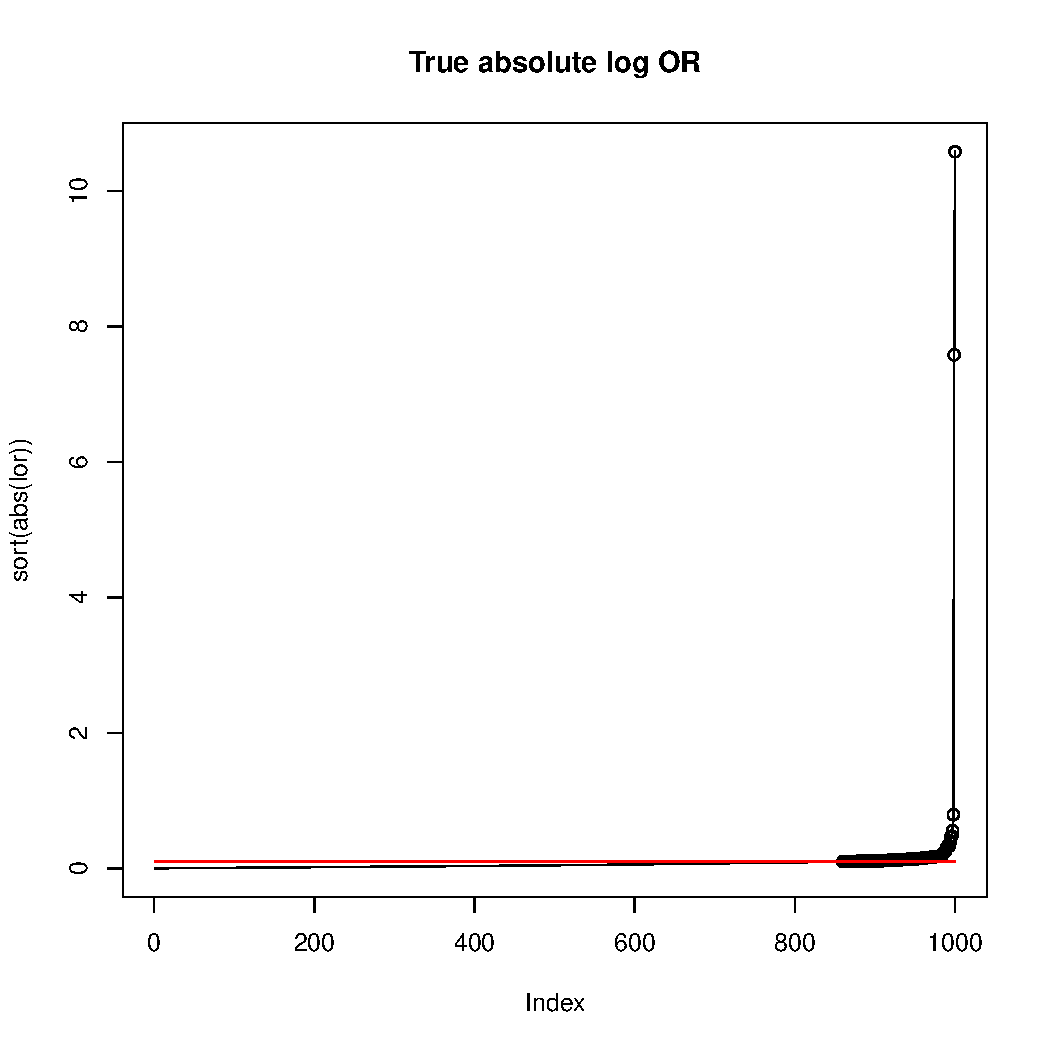
\includegraphics[scale=0.25]{impute_g1.pdf}
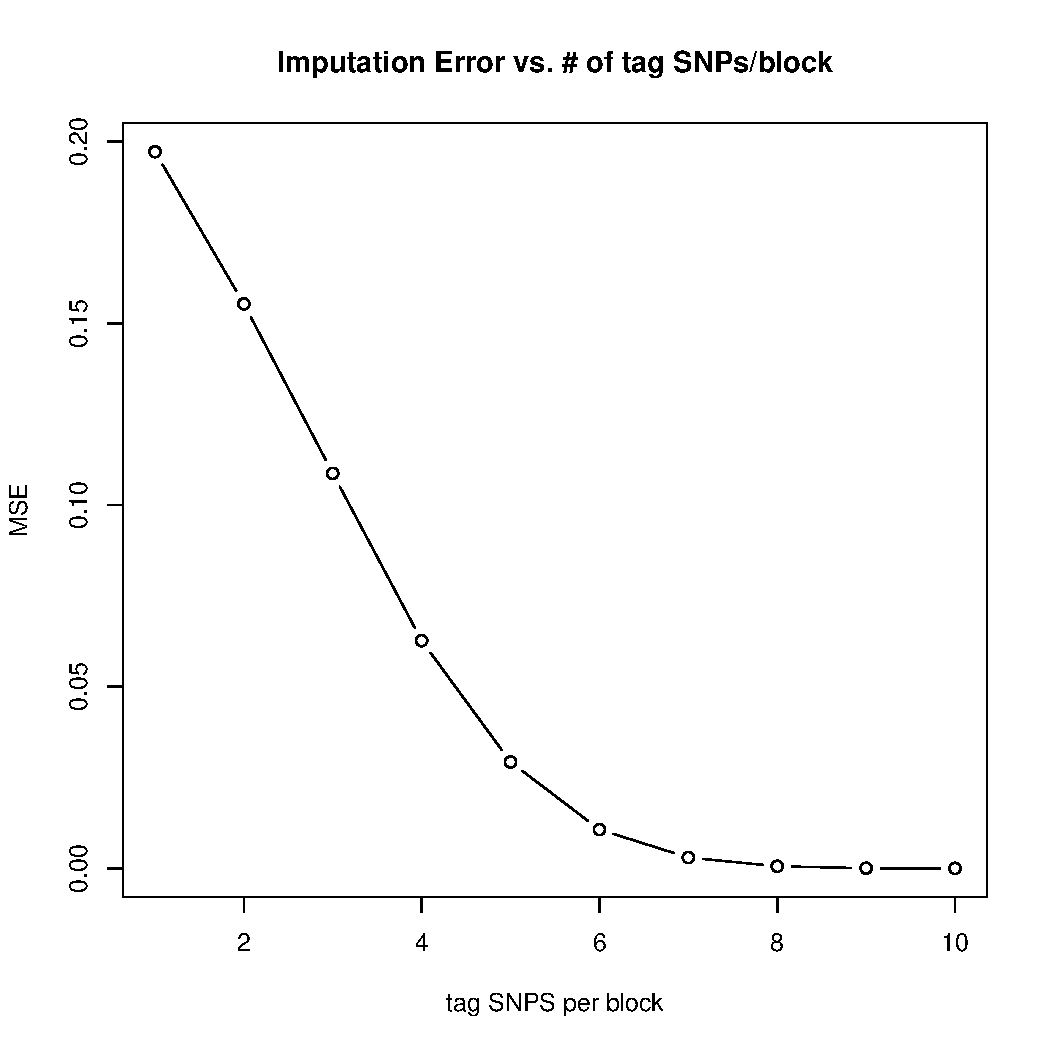
\includegraphics[scale=0.25]{impute_g2.pdf}
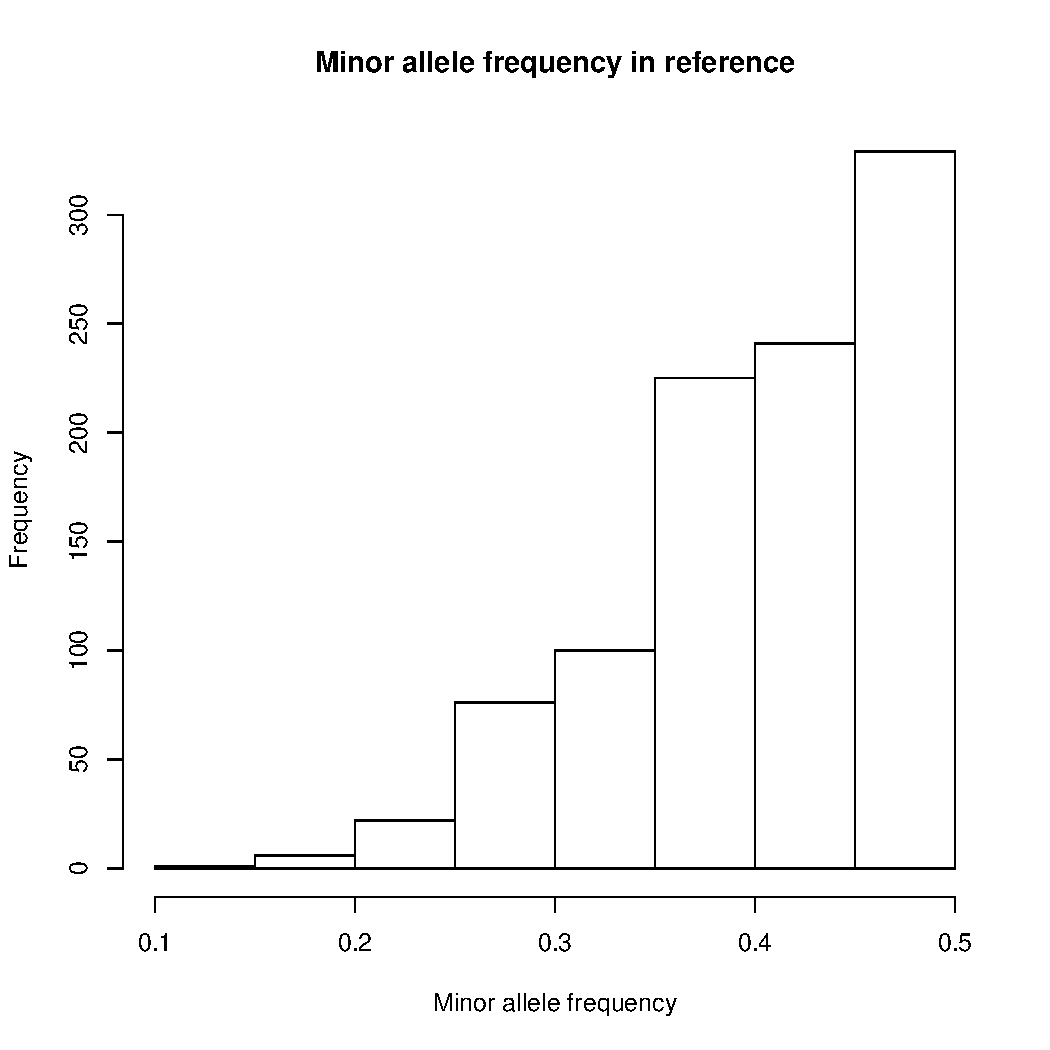
\includegraphics[scale=0.25]{impute_g3.pdf}
\caption{\emph{Left} (i). True absolute log odds ratios of SNPs (sorted)  \emph{Center} (ii) Imputation error vs number of tag
  SNPs per haplotype Block.  Error is measured by average squared
  error. \emph{Right} (iii) Minor allele frequency in reference}
\end{figure}

Using the full reference panel with no errors, and 4 tag SNPs per
block, we have significant discordance between true log odds ratios
and asymptotic imputed data log odds ratios (Figure 5(i)), with 63
systematically induced false positives.
However, we will see that given a realistic sample size,
the false positive rate may be much lower.

In one run, we use $L=10000$ cases and the same number of controls,
with 4 tag SNPs per block.
Figures 5(ii) and (iii) show the false discovery proportion (fdp) curves
for genotyped data and imputed data, respectively.
Notable is the fact that the fdp curve for imputed data is rougher,
a trend that becomes increasingly evident when the sample size
increases.

\begin{figure}[h]
\centering
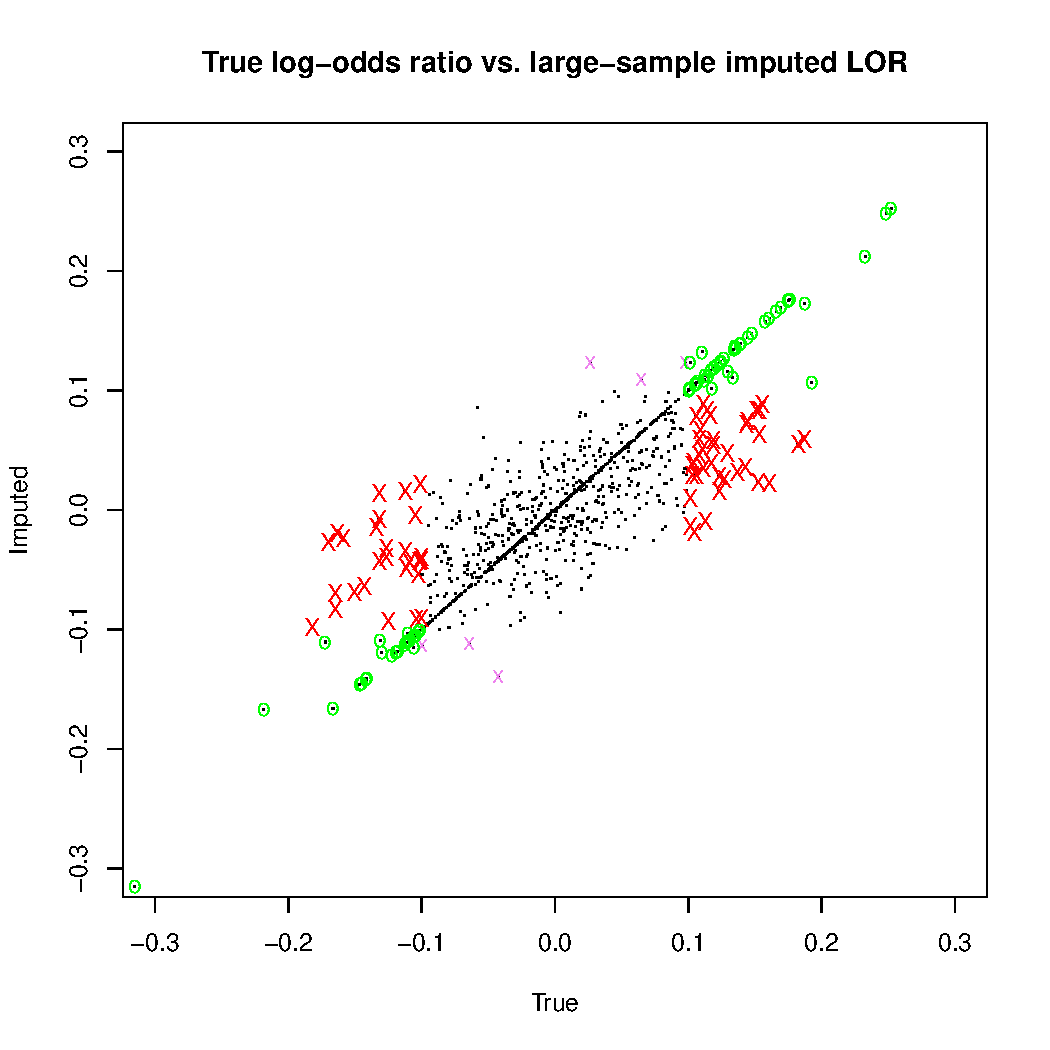
\includegraphics[scale=0.25]{impute_g4.pdf}
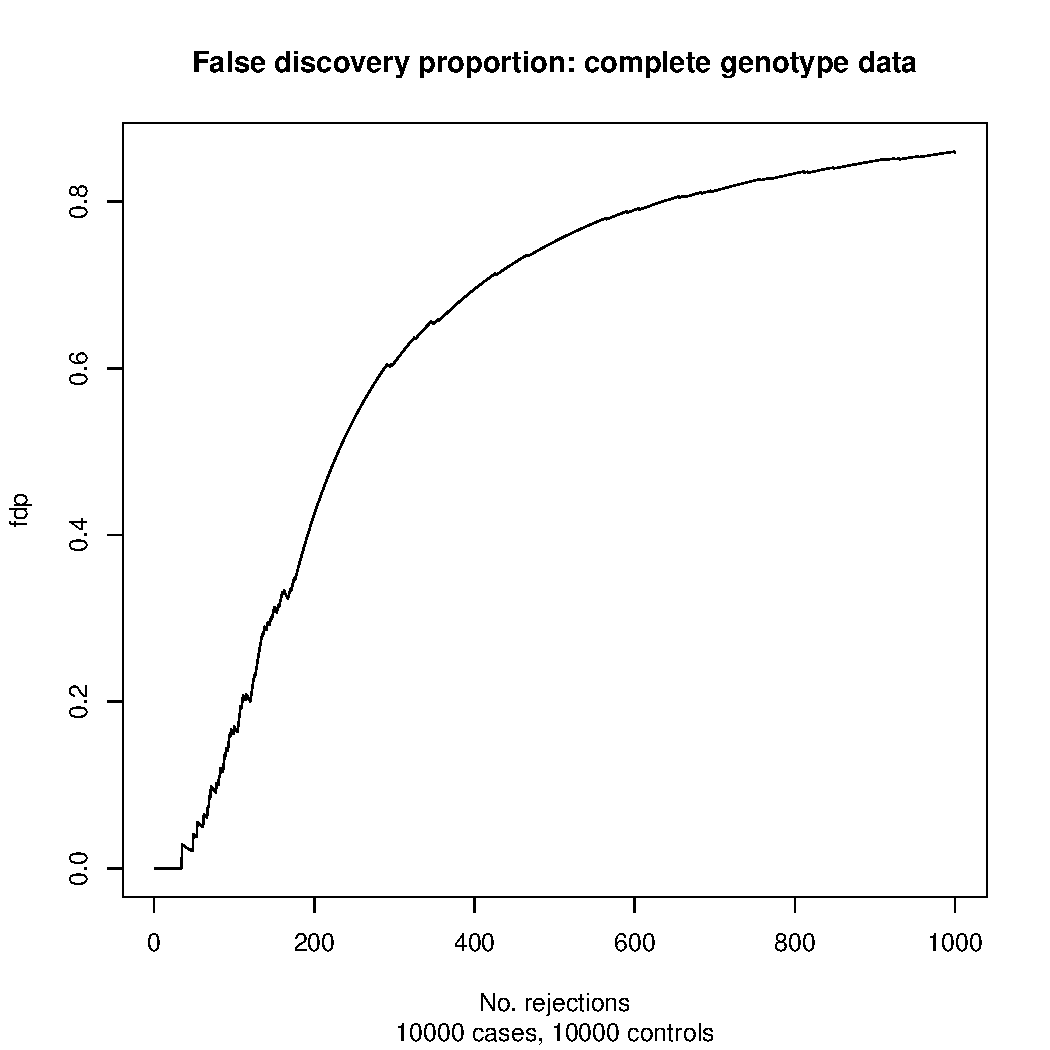
\includegraphics[scale=0.25]{impute_g5.pdf}
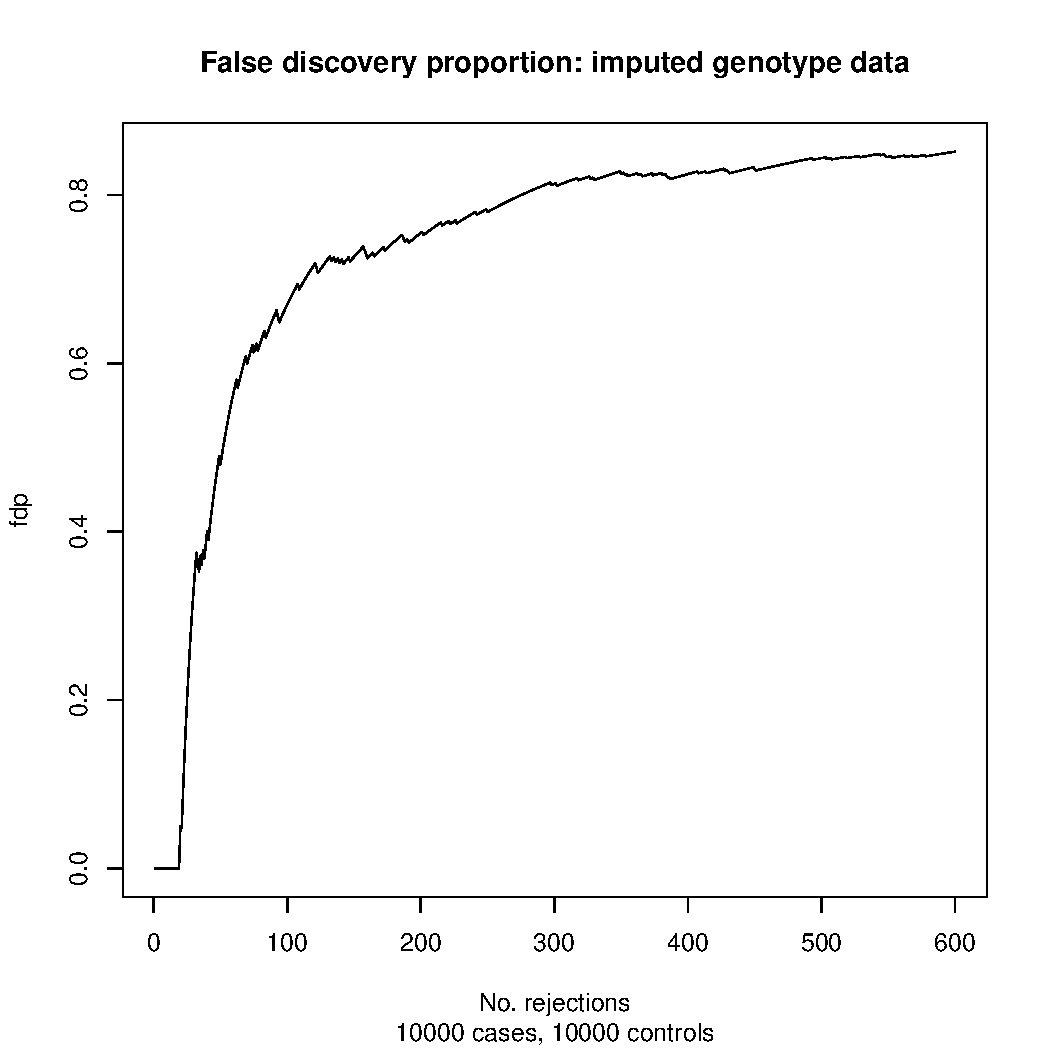
\includegraphics[scale=0.25]{impute_g6.pdf}
\caption{\emph{Left} (i). True log odds ratios of SNPs vs. asymptotic
imputed log odds ratios, 4 tag SNPS/block.  Green circles=true positives, violet
crosses=false negatives, red crosses=false positives.  \emph{Center}
(ii) False discovery proportion of genotyped data, $L=1000$
 \emph{Right} (iii) False discovery proportion of imputed data,
 $L=1000$, 4 tag SNPS/block}
\end{figure}

We set $L_{val} = 1000$, and false discovery rate threshold to
$q=0.2$.
We compare the following procedures
\begin{itemize}
\item BH(q) on the complete genotyped data
\item BH(q) on the data imputed using the given tag SNPs
\item Our method on the imputed data
\end{itemize}
The following table shows the results of a few repeated runs.
Recall $R$ is the number of rejections, $V$ the number of false
rejections, and $fdp = V/R$.

\noindent
\begin{tabular}{|c|ccc|ccc|ccc|}
\hline
Run & Full data $R$ & $V$ & fdp & Imputed $R$ & $V$ & fdp & Our method
$R$ & $V$ & fdp\\
1 & 22 & 0 & 0 & 11 & 0 & 0 & 8 & 0 & 0\\
2 & 20 & 0 & 0 & 9 & 0 & 0 & 7 & 0 & 0\\
3 & 20 & 0 & 0 & 10 & 0 & 0 & 8 & 0 & 0\\
\hline
\end{tabular}
In summary, neither the naive method nor our method makes
any false rejections, though our method has less power.
\[\]
\noindent\emph{Increased sample size}

Increasing the sample size a hundred fold to $L=1000000$ and $L_{val}=10000$,
problems start to occur for the naive method.
However, our method continues to be quite
conservative.

\noindent
\begin{tabular}{|c|ccc|ccc|ccc|}
\hline
Run & Full data $R$ & $V$ & fdp & Imputed $R$ & $V$ & fdp & Our method
$R$ & $V$ & fdp\\
1 & 111 & 0 & 0 & 29 & 6 & 0.21 & 13 & 1 & 0.07\\
2 & 112 & 0 & 0 & 29 & 6 & 0.21 & 13 & 1 & 0.07\\
3 & 111 & 0 & 0 & 28 & 6 & 0.21 & 14 & 1 & 0.07\\
\hline
\end{tabular}
Notice that at this sample size, the sampling error has
little influence compared to the systematic bias
induced by the imputation procedure.
\[\]
\noindent\emph{Incomplete reference panel}

Return to $L=10000$ and $L_{val}=1000$, but this time construct
the reference panel by a subsample of size 25.
Systematically induced false positives increase to 75
while asymptotically detectible true positives decrease to 19.
Power for both the naive method drops slightly,
more for our method.
Yet no false rejections are made.

\noindent
\begin{tabular}{|c|ccc|ccc|ccc|}
\hline
Run & Full data $R$ & $V$ & fdp & Imputed $R$ & $V$ & fdp & Our method
$R$ & $V$ & fdp\\
1 & 25 & 0 & 0 & 7 & 0 & 0 & 6 & 0 & 0\\
2 & 25 & 0 & 0 & 6 & 0 & 0 &6 & 0 & 0\\
3 & 30 & 0 & 0 & 7 & 0 & 0 &0 & 0 & 0\\
\hline
\end{tabular}
\[\]
\noindent\emph{Incomplete reference, more tag SNPs}

Here is a scenario in which the effects of Pattern I manifest.
Return to $L=10000$ and $L_{val}=1000$, and 
As in the last section, our reference panel is a subsample of size 25 of the true
reference panel, but now increase the number of
tag SNPs to 6 per block.

\begin{figure}[h]
\centering
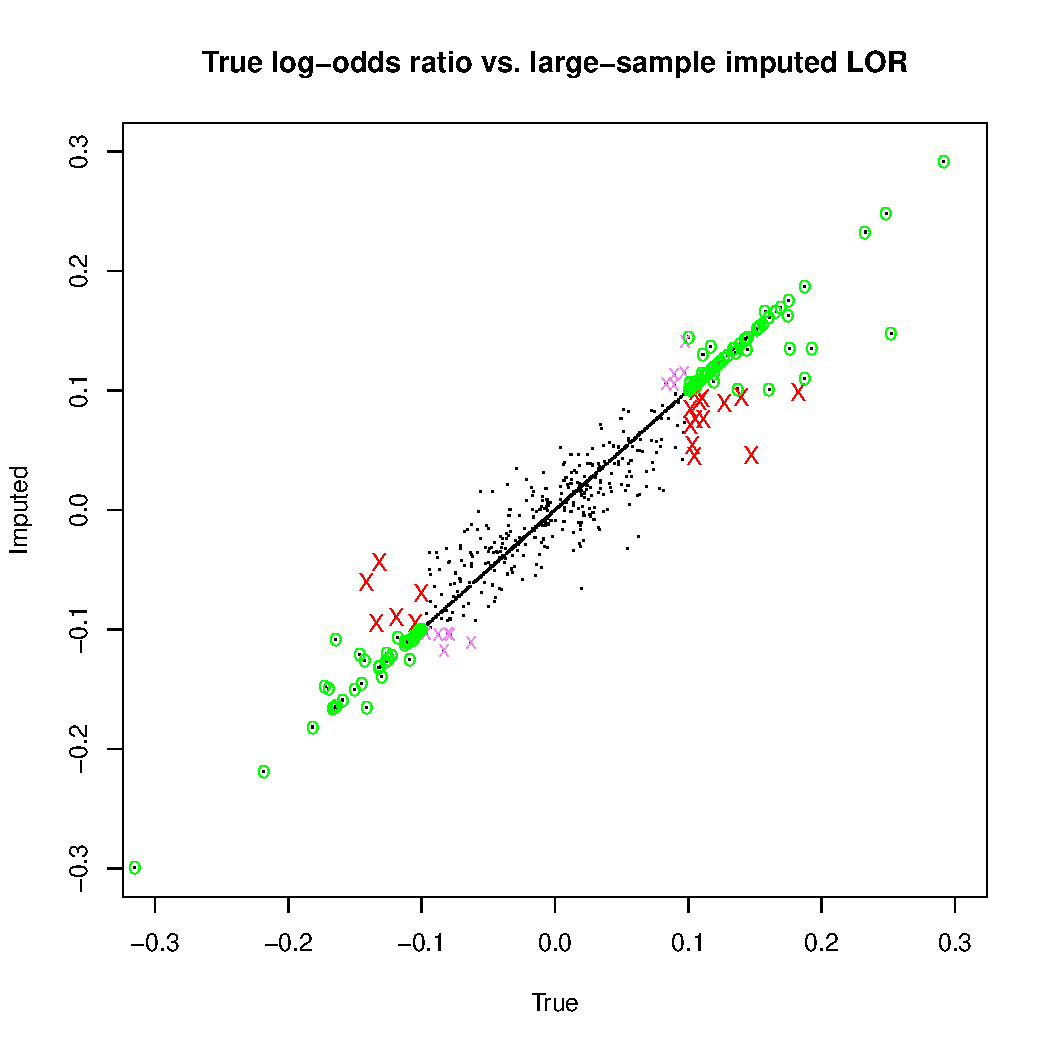
\includegraphics[scale=0.25]{impute_g7.pdf}
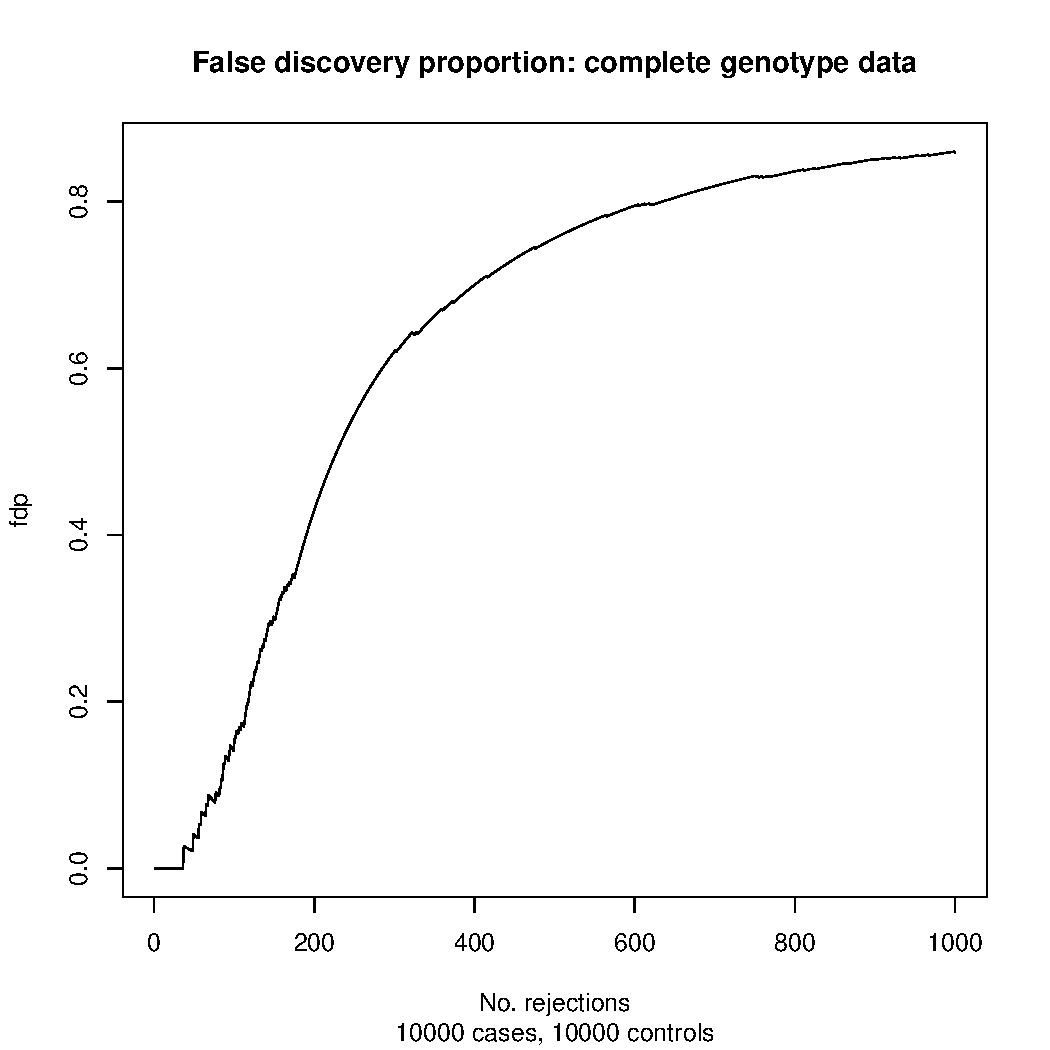
\includegraphics[scale=0.25]{impute_g8.pdf}
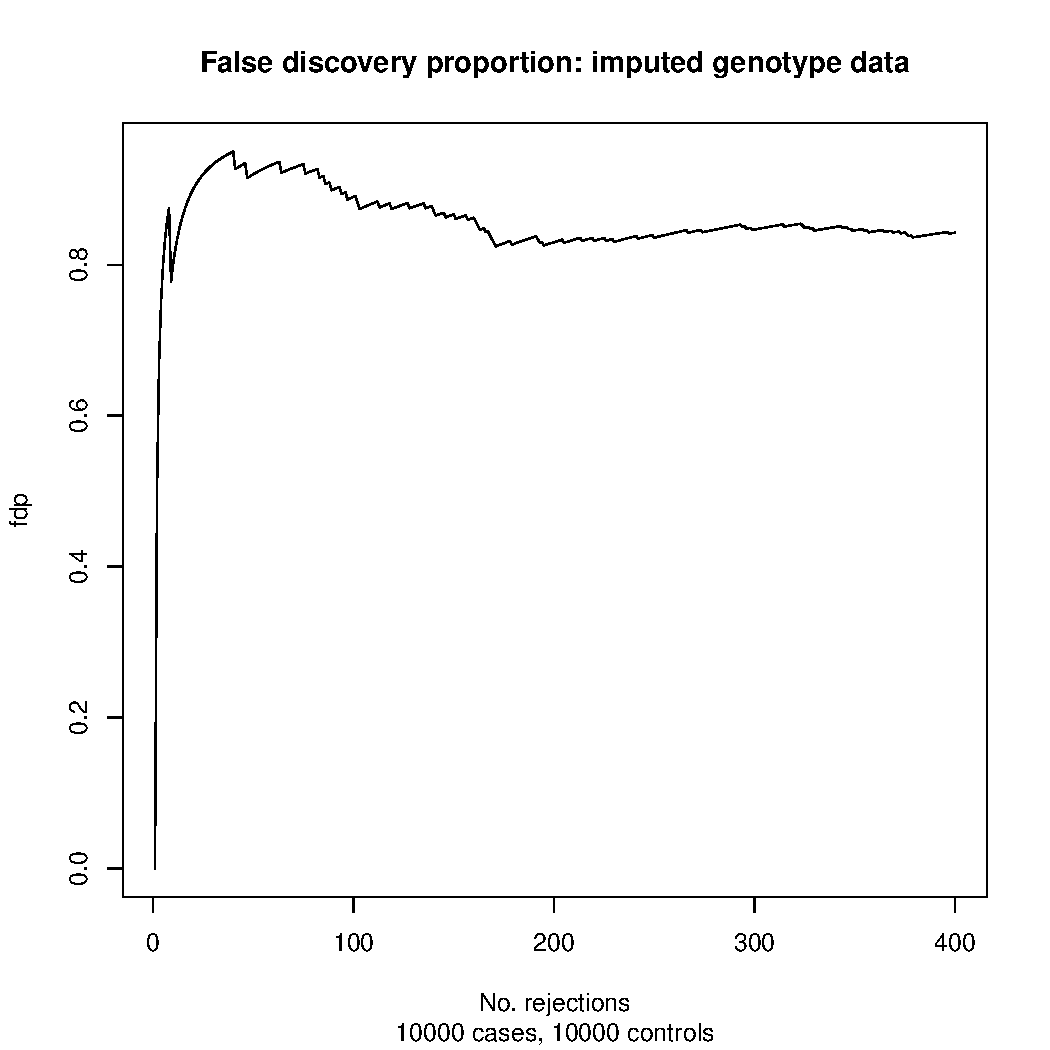
\includegraphics[scale=0.25]{impute_g9.pdf}
\caption{\emph{Left} (i). True log odds ratios of SNPs vs. asymptotic
imputed log odds ratios, 6 tag SNPS/block.  Green circles=true positives, violet
crosses=false negatives, red crosses=false positives.  \emph{Center}
(ii) False discovery proportion of genotyped data, $L=1000$
 \emph{Right} (iii) False discovery proportion of imputed data,
 $L=1000$, 6 tag SNPS/block}
\end{figure}

  The large-sample number of false positives
due to imputation errors reduces to 19, and the number of true
positives detectible in the imputation data increases to 44.
Yet surprisingly, the false positive rates rise for the naive method.

\noindent
\begin{tabular}{|c|ccc|ccc|ccc|}
\hline
Run & Full data $R$ & $V$ & fdp & Imputed $R$ & $V$ & fdp & Our method
$R$ & $V$ & fdp\\
1 & 21 & 0 & 0 & 7 & 6 & 0.85 & 0 & 0 & 0\\
2 & 30 & 0 & 0 & 11 & 9 & 0.81 &0 & 0 & 0\\
3 & 25 & 0 & 0 & 9 & 8 & 0.88 &0 & 0 & 0\\
\hline
\end{tabular}

This phenomenon can be explained, however.
We have removed additional tag SNPs
from the list of SNPs to be be tested and thus depleted the data
of many strong signals.
On the other hand, having more tag SNPs, up to a certain point,
increases the prospect of Pattern I (\S 3.1) occurring,
since Pattern I depends on the existence of two haplotypes
which are indistinguishable given the typed SNPs,
but which are distinguished from the other haplotypes
in the population.
Figure 6 provides a comparison with with Figure 5.

While the naive method is plagued with almost as many false
discoveries as true ones,
our method controls the type I error by making no rejections.

\section{Discussion}

Our simulations show that in certain conditions,
the naive method for testing imputed data can
have some degree of robustness against incomplete reference data.
However, rather counterintuitively, a large sample size,
and a relatively large number of tag SNPs can lead to dramatically
increased type I error rates for naive testing of associations
based on imputed data.

Given the difficulty of gauging one's vulnerability
to increased type I error from using imputed data,
it would be prudent to obtain some form of additional validation data
to check for the prevalence of systematic error induced by imputation.
Our method is a formal way to do this--
it has some degree of guaranteed type I error control,
but it requires huge sample sizes to be truly effective, and
is often overconservative to the extreme in common situations.

It remains for future work to develop a method which can control
type I error for imputed data, and yet remain competitive against
the naive methods in situations where excessive caution is unwarranted.

\bibliographystyle{abbrv}
\bibliography{gwas,books}

\end{document}



